\documentclass[12pt, titlepage]{article}

\usepackage{booktabs}
\usepackage{tabularx}
\usepackage{graphicx}
\usepackage{enumitem}
\usepackage{hyperref}
\usepackage{graphicx}
\hypersetup{
    colorlinks,
    citecolor=black,
    filecolor=black,
    linkcolor=red,
    urlcolor=blue
}
\usepackage[round]{natbib}

\title{SE 3XA3: Software Requirements Specification\\PokerProject}

\author{Team \#12, Team Name
        \\ Safwan Hossain, hossam18
        \\ Eamon Earl, earle2
        \\ Tyler Magarelli, magarelt
}

\date{\today}


\begin{document}

\maketitle

\pagenumbering{roman}
\tableofcontents
\listoftables
\listoffigures

\begin{table}[bp]
\caption{\bf Revision History}
\begin{tabularx}{\textwidth}{p{3cm}p{2cm}X}
\toprule {\bf Date} & {\bf Version} & {\bf Notes}\\
\midrule
2022-02-11 & 1.0 & \\
\bottomrule
\end{tabularx}
\end{table}

\newpage

\pagenumbering{arabic}

This document describes the requirements for a client-server Poker project that will be programmed using Java.

\section{Project Drivers}

\subsection{The Purpose of the Project}
Poker is a world renowned card game in which players must use their understanding of probability,
wit and deceptive strategy to best their opponents and win money. While poker is very commonly
played face-to-face on a table, the goal of this project is to make a variety of poker game-types easily
accessible from anywhere, without betting, and for all ages. The current software we begin with sets the framework for randomizing
poker hands and analyzing them, and by expanding upon this foundation we will be able to develop a complete poker
experience.
\subsection{The Stakeholders}

\subsubsection{The Developers}
As our project will be created in a Java environment, the software developers are provided the correct environment to be able to easily adapt and tailor the software towards a simple yet effective interface with high cohesion and low coupling,
while providing the user an easy way to play whenever desired with very little initial setup. The developers are also responsible for testing the program and internally managing the project.
\subsubsection{The Customers}
The primary stakeholder to consider during the development process is the subgroup that will be directly using and interfacing with the finished product; the customer. Our main goal for this relationship is to cater to them a full poker experience, and an easy way to engage in this neglected sport with no financial cash flow required from them for the purposes of betting. We will also be providing online play, via private online lobbies, so that the customer can play with their friends. Random match-making could be a later implementation to further improve the user experience, but this goal will lay outside the scope of the project, and will be discussed later on in this document.
\subsubsection{Other Stakeholders}
For the purpose of this project, the publisher is considered to be the Department of Computing and Software at McMaster University, wherein their input will be queried and provided throughout the documentation and development process, and will most notably affect this SRS at revision 1, which will be finalized by March 18th. 
\subsection{Mandated Constraints}
The scope of this project will, to some degree, be inherently described by the constraints, and as such they will be listed and discussed first. 

\bigskip

Description: Our software will be able to run on any machine that is capable of running JVM on their system.

Rationale: Any semi-modern local computing device has the capability to run java programs, and as such we will be keeping our demographic of eligible customers as large as possible.

Fit Criterion: Our program will be entirely enclosed within java software and architecture, including the server implementation. Our UI will be text based and represented in the console. 

\bigskip

Description: Our program will not involve gambling using real-world currency.

Rationale: Including this feature would conflict with the constraints specified by our publishers, and would greatly extend the scope of this project, to a degree that would require far more resources to complete.

Fit Criterion: Poker chips will be rewarded equally to all players for any game, and will merely be represented in data; we wish to focus on the practical and mental benefits of the game of poker, not the financial deficits.  

\subsection{Naming Conventions and Terminology}
\subsubsection{Definitions}
\begin{itemize}
    \item \textbf{Chips} - The currency of the game.
    \item \textbf{Pot} - The collective pool of chips that all the players bet on.
    \item \textbf{Hand} - A combination of a player's pair of cards and the cards on a table.
    \item \textbf{Bet} - To increase the amount of chips needed for the round to end.
    \item \textbf{Check} - To not bet without folding.
    \item \textbf{Call} - A bet that is the equal amount to the bet made prior. A player who calls frequently without raising or folding is known as a “calling station”.
    \item \textbf{Raise} - To bet higher than an existing bet.
    \item \textbf{Fold} - To forfeit any bets made and surrender your cards within a hand.
    \item \textbf{All-In} - The act of risking all of your chips on one single hand.
\end{itemize}

\subsection{Environment}

    \begin{figure}
        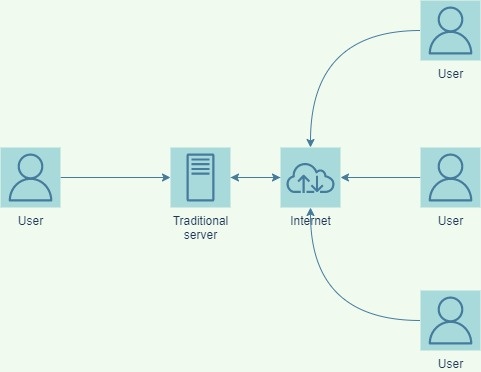
\includegraphics[width=15cm]{implementation_environment (1).jpg}
        \caption{Server Architecture}
    \end{figure}

\bigskip

Above, we see the general architecture of the online aspect of the game, where each user will access a shared server via their respective internet connections. Once again, this server will be low fidelity and will be created entirely within Java. 

\subsection{Architecture}

We have decided on the Model-View-Controller (MVC) architecture, as it is well geared towards playable games. It also gears itself towards designing for change in the sense of the generality required to implement other game modes in the future; they would use easily use the same model, as they are all played with one deck of cards and one hand per player, and would only require a specific controller to script the game (and possibly some additional methods in the view). This allows future developers to leave the entirety of the data untouched - an exceptionally valuable trait for developing pre-existing software. 

\begin{figure}
    \centering
    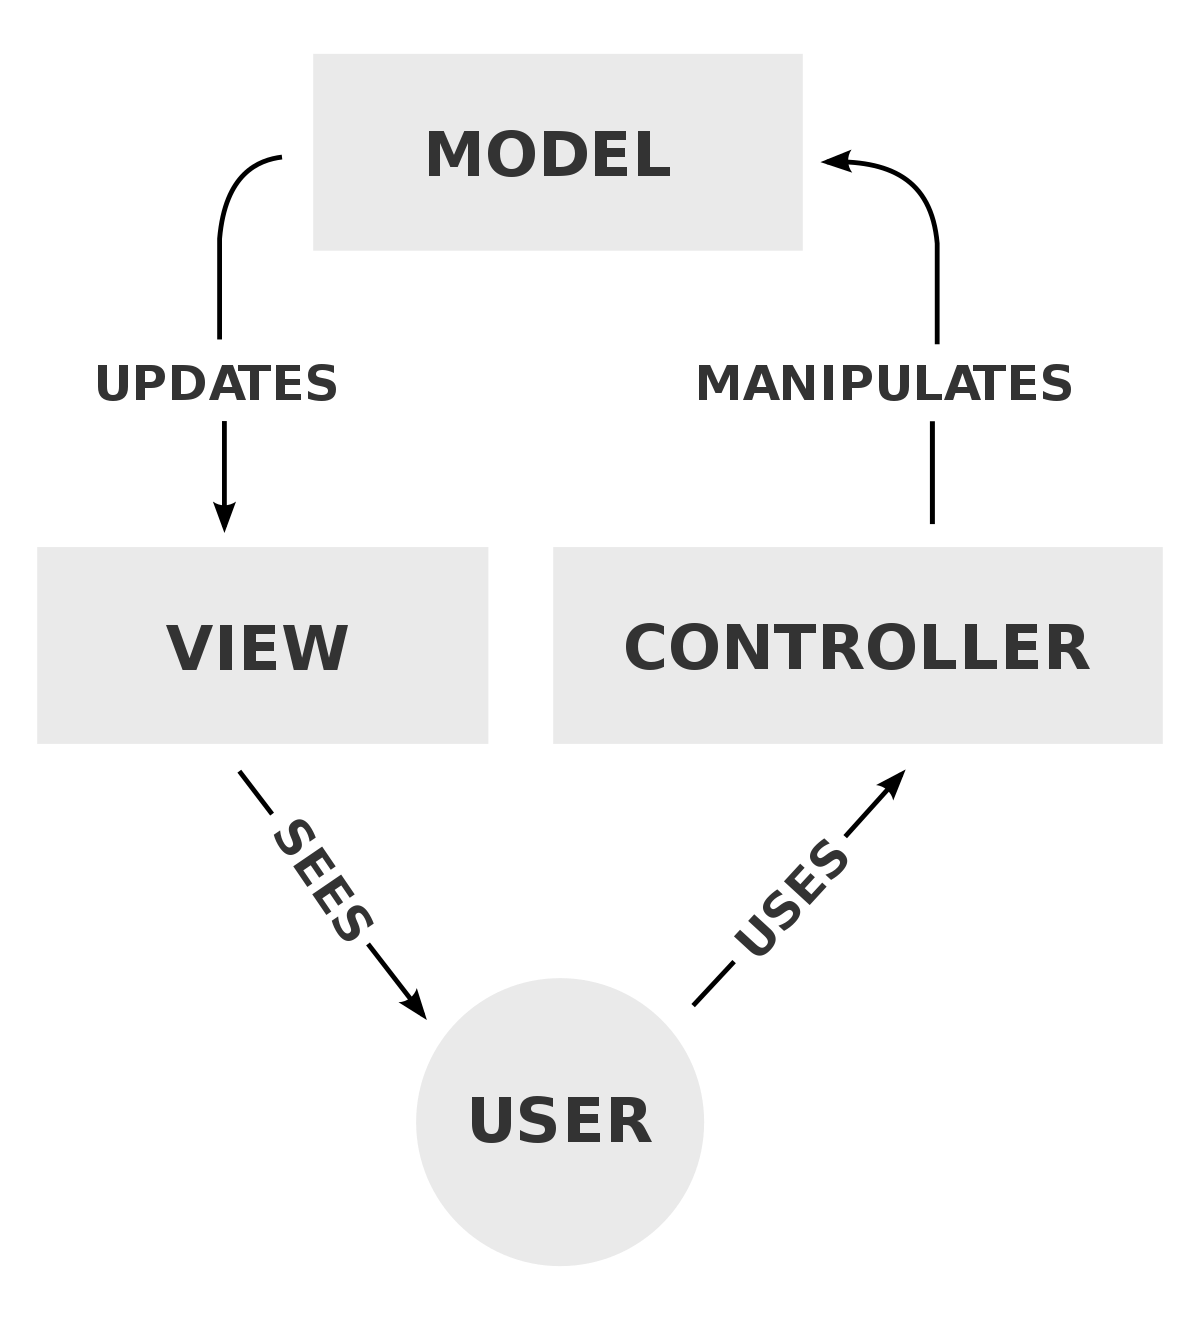
\includegraphics[width=10cm]{MVC-Process.svg.png}
    \caption{MVC Architecture}
\end{figure}

\section{Functional Requirements}

\subsection{The Scope of the Work and the Product}

    The scope of this project is contained to being held within java framework, and is limited by the deadlines and relatively tight schedules of the students who take the roles of developers. We will implement one main poker game mode, and do so in such a way that adding more in future iterations of the project would be straightforward, and would not require reconfiguration of the existing architecture, merely additional controllers; thus designing for generality. As we will be implementing "Texas Hold'em" as the initial game mode, the program will be inherently a multiplayer experience, with offline local multiplayer and online multiplayer as well. The servers for online multiplayer will be implemented with low fidelity and bandwidth, as it is known by the project managers that at this point we are not designing for a large player base, and the project is not due to hit markets during the current project life cycle.
    
    As previously discussed, using real currency for the betting process is outside of the scope of this project.
    

\subsection{Functional Requirements}
    \begin{enumerate}[label=FR\arabic*.]
        \item The user shall be able to generate a unique alphanumeric code that will allow other users to join their lobby.
        \item The user shall be able to join lobbies by entering in a valid alphanumeric code.
        \item The user shall be able to perform at most one of the following actions during their turn: fold, check, call, bet, raise.
        \item The system shall automatically fold any player that does not make a move within the allotted period of time during their turn.
        \item A game shall have a specified maximum amount of players.
        \item A game shall have a specified minimum amount of players.
        \item The system shall be able to identify the correct card ranking for a player's hand.
        \item The system shall carry a virtual standard deck of cards, consisting of 52 unique cards.
        \item The system shall shuffle its deck of cards before every game.
        \item At the start of the game, the system shall give a random player the role of the dealer. Note that this is just a title and the system will deal the cards, not the player.
        \item Each round, the first player to the immediate left of the dealer shall be given the role of small blind.
        \item Each round, the first player to the immediate left of the small blind shall be given the role of big blind.
        \item The system shall take half of a specified amount of money from the small blind and add it to the money pool in the beginning of the round.
        \item The system shall take a specified amount of money from the big blind as it did from the small blind and add it to the money pool in the beginning of the round.
        \item The system shall give each player on the table 2 cards in the beginning of the first round.
        \item The player to the immediate left of the big blind shall be given the first turn.
        \item The system shall allow at most one user to have a turn any time during a game.
        \item After a player is done their turn, the player to the immediate left of them shall be given a turn.
        \item Once every player has either bet the same amount or decided to fold the round ends.
        \item After the first round, the system shall present three cards from its deck face up to all of the players.
        \item After the second round, the system shall present one card from its deck face up to all of the players.
        \item After the third round, the system shall present one card from its deck face up to all of the players.
        \item After the fourth round, each player shall be forced to present their cards face up to all the other players.
        \item During the fifth round, the player with the highest hand ranking will win the pot.
        \item If the highest hand ranking belongs to more than one player, then the pot will be split among the highest ranking players.
        \item After the fifth round, all cards will be collected and the game will start again from round one.
        \item The system shall give each player a specified amount of money when they join.
        \item If a player loses all their money they will be kicked from the table.
        \item If a player does not have enough money to call a bet they will be allowed to go all in.
        \item If a player does not have enough money to pay for big or small blind, they will be allowed to go all in.
        
    \end{enumerate}
\section{Non-functional Requirements}

\subsection{Look and Feel Requirements}
    Because the system will be currently be using the console and optionally in the future use a GUI this requirement is not applicable. 
\subsection{Usability and Humanity Requirements}
    \subsubsection{Ease of Use Requirements}
        \label{ssub:ease_of_use_requirements}
        % Begin SubSubSection
        \begin{enumerate}[label=UH\arabic*.]
            \item The user should be able to perform their desired action in no more than 3 clicks/menus.
        \end{enumerate}
        

\subsection{Performance Requirements}
    \subsubsection{Speed and Latency Requirements}
    \begin{enumerate}[label=PR\arabic*.]
        \item Any interface between a user and the system shall have a maximum response time of 500ms.
        \item The maximum time to boot the game on any system shall be less than 2 minutes.
    \end{enumerate}
    \subsubsection{Reliability and Availability Requirements}
    \begin{enumerate}[label=PR\arabic*.]
        \item The system shall run whenever the user desires to open the application.  
    \end{enumerate}
    \subsubsection{Robustness or Fault-Tolerance Requirements}
    \begin{enumerate}[label=PR\arabic*.]
        \item The system shall be designed to operate on a highly robust level.
    \end{enumerate}
    \subsubsection{Capacity Requirements}
    \begin{enumerate}[label=PR\arabic*.]
        \item Each lobby / local game can have at most 6 individual players. 
    \end{enumerate}
    \subsubsection{Scalability or Extensibility Requirements}
    \begin{enumerate}[label=PR\arabic*.]
        \item The system shall be able to update through software updates that are issued by the developers.
    \end{enumerate}
    \subsubsection{Longevity Requirements}
    \label{ssub:longevity_requirements}
     % Begin SubSubSection
    \begin{enumerate}[label=PR\arabic*.]
        \item The product will be developed under the heuristics of designing for change via generality.  
    \end{enumerate}
    % End SubSubSection
\subsection{Operational and Environmental Requirements}
    \subsubsection{Expected Physical Environment}
    \label{ssub:expected_physical_environment}
    % Begin SubSubSection
    \begin{enumerate}[label=OE\arabic*.]
        \item The system will be expected to be installed onto the user's local machine.
    \end{enumerate}
    % End SubSubSection
    
\subsection{Maintainability and Support Requirements}
    
    \subsubsection{Supportability Requirements}
    \label{ssub:supportability_requirements}
    % Begin SubSubSection
    \begin{enumerate}[label=MS\arabic*.]
        \item The system should be able to be update through software patches issued by the developers.
    \end{enumerate}
    % End SubSubSection
    
    \subsubsection{Adaptability Requirements}
    \label{ssub:adaptability_requirements}
    % Begin SubSubSection
    \begin{enumerate}[label=MS\arabic*.]
        \item The system should be able to be extended by adding more features by the developers.
    \end{enumerate}
    % End SubSubSection
    
    % End SubSection

\subsection{Security Requirements}
    \subsubsection{Access Requirements}
    \label{ssub:access_requirements}
    % Begin SubSubSection
    \begin{enumerate}[label=SR\arabic*.]
        \item The alphanumeric codes for lobby creation and access will be encrypted / generated by some means such that unwanted players cannot easily join.
    \end{enumerate}
    % End SubSubSection
    
    \subsubsection{Privacy Requirements}
    \label{ssub:privacy_requirements}
    % Begin SubSubSection
    \begin{enumerate}[label=SR\arabic*.]
        \item The lobby creators will have the option to kick players out of a lobby before the game commences.
    \end{enumerate}
    % End SubSubSection
\subsection{Cultural Requirements}
N/A.
\subsection{Legal Requirements}
N/A.
\subsection{Health and Safety Requirements}
N/A.
\section{Project Issues}
N/A.
\subsection{Open Issues}
N/A.
\subsection{Off-the-Shelf Solutions}
Some of these off the shelf solutions for the risks may include:

\begin{enumerate}
    \item Hostinger - a cheap cloud based virtual server with varying payment plans for different requirements
    \item InterServer - a fairly priced server for hosting powerful Java applications (could be more sophisticated than we need) 
    \item Hostwinds - requires more knowledgeable server developer, but grants more in-depth control and customization, with great service almost internationally
\end{enumerate}

\subsection{New Problems}
N/A.
\subsection{Tasks}
N/A.
\subsection{Migration to the New Product}
N/A.
\subsection{Risks}
Some technical risks that need to be weighed out are the implications of running a low fidelity java server off of one of the developer's local machines. This will be something that needs to be tested during the proof of concept such that we can see if our intended number of concurrent online players is feasible under such conditions, else we may wish to consider some off-the-shelf solutions for our server. 

\subsection{Costs}
Costs will be considered at a later date once the server is implemented.
\subsection{User Documentation and Training}
N/A.
\subsection{Waiting Room}
N/A.
\subsection{Ideas for Solutions}
N/A.
\bibliographystyle{plainnat}

\bibliography{SRS}

\newpage

\section{Appendix}

\subsection{Symbolic Parameters}

\end{document}